\documentclass{article}%
\usepackage[T1]{fontenc}%
\usepackage[utf8]{inputenc}%
\usepackage{lmodern}%
\usepackage{textcomp}%
\usepackage{lastpage}%
\usepackage[head=40pt,margin=0.5in,bottom=0.6in]{geometry}%
\usepackage{graphicx}%
%
\title{\textbf{Las dos versiones oficiales sobre la muerte de Fernando Albán}}%
\author{EL NACIONAL WEB}%
\date{08/10/2018}%
%
\begin{document}%
\normalsize%
\maketitle%
\textbf{URL: }%
http://www.el{-}nacional.com/noticias/sucesos/las{-}dos{-}versiones{-}oficiales{-}sobre{-}muerte{-}fernando{-}alban\_254902\newline%
%
\textbf{Periodico: }%
EN, %
ID: %
254902, %
Seccion: %
Sucesos\newline%
%
\textbf{Palabras Claves: }%
NO\_TIENE\newline%
%
\textbf{Derecho: }%
1.1, %
Otros Derechos: %
1.2, 1.10, %
Sub Derechos: %
1.1.1.3, 1.2.2, 1.10.1\newline%
%
\textbf{EP: }%
NO\newline%
\newline%
%
\textbf{\textit{Néstor Reverol informó que el subdirector del Cicpc y un equipo multidisciplinario seran los responsables de la investigación del evento~}}%
\newline%
\newline%
%
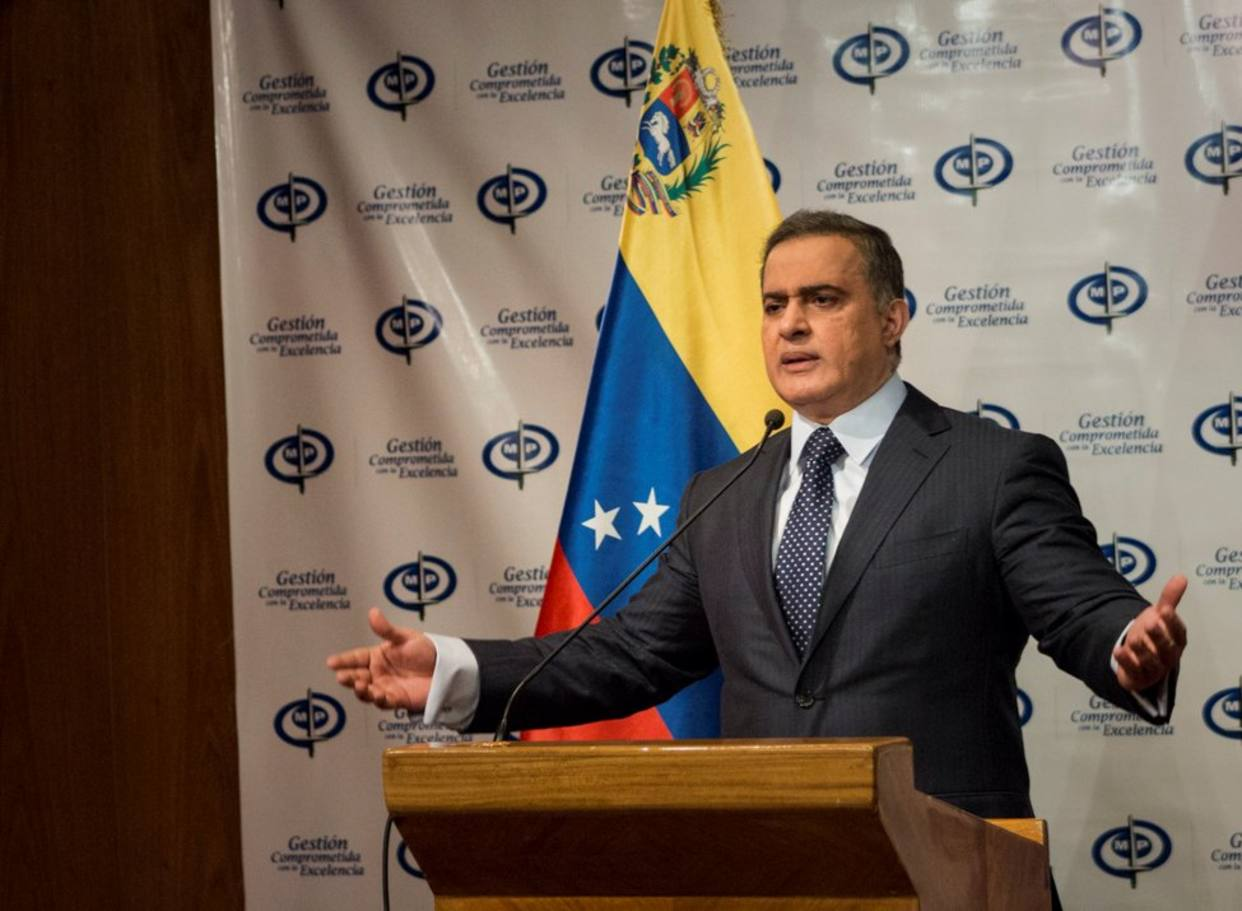
\includegraphics[width=300px]{228.jpg}%
\newline%
%
Tarek William Saab, fiscal general designado por la asamblea nacional constituyente, confirmó la muerte del concejal Fernando Albán en la sede del Servicio Bolivariano de Inteligencia (Sebin) en Plaza Venezuela.%
\newline%
%
Hay dos versiones del evento dadas por el gobierno, la del fiscal general designado por la asamblea nacional constituyente y la de Néstor Luis Reverol, ministro de Interior,~Justicia y Paz.%
\newline%
%
De acuerdo con Saab, el concejal pidió ir al baño y luego se lanzó desde el piso 10 del establecimiento. Reverol por su parte, indicó que el político estaba en la sala de~espera para ser trasladado a los Tribunales cuando se quitó la vida.%
\newline%
%
El ministro informó que el subdirector del Cuerpo de Investigaciones Científicas Penales y Criminalísticas (Cicpc)~y un equipo multidisciplinario seran los responsables de la investigación del suceso.%
\newline%
%
El concejal del municipio Libertador fue detenido por funcionarios del Sebin este viernes en el Aeropuerto de Internacional Simón Bolívar, ubicado en Maiquetía, estado Vargas.%
\newline%
%
\end{document}